\section{Model and Methods}
\label{sec:model-methods}

This section documents the Level 1.2/1.2b model and discovery methodology
in the detail needed to interpret \cref{sec:level12,sec:level12b}.
\Cref{sec:appendix-odd} gives a compact ODD-style (Overview, Design
concepts, Details; \cite{grimm2006standard,grimm2010odd,grimm2020odd})
summary; full field-level documentation is in the source repository's own
configuration reference (\cref{sec:reproducibility}).

\begin{figure}[htbp]
\centering
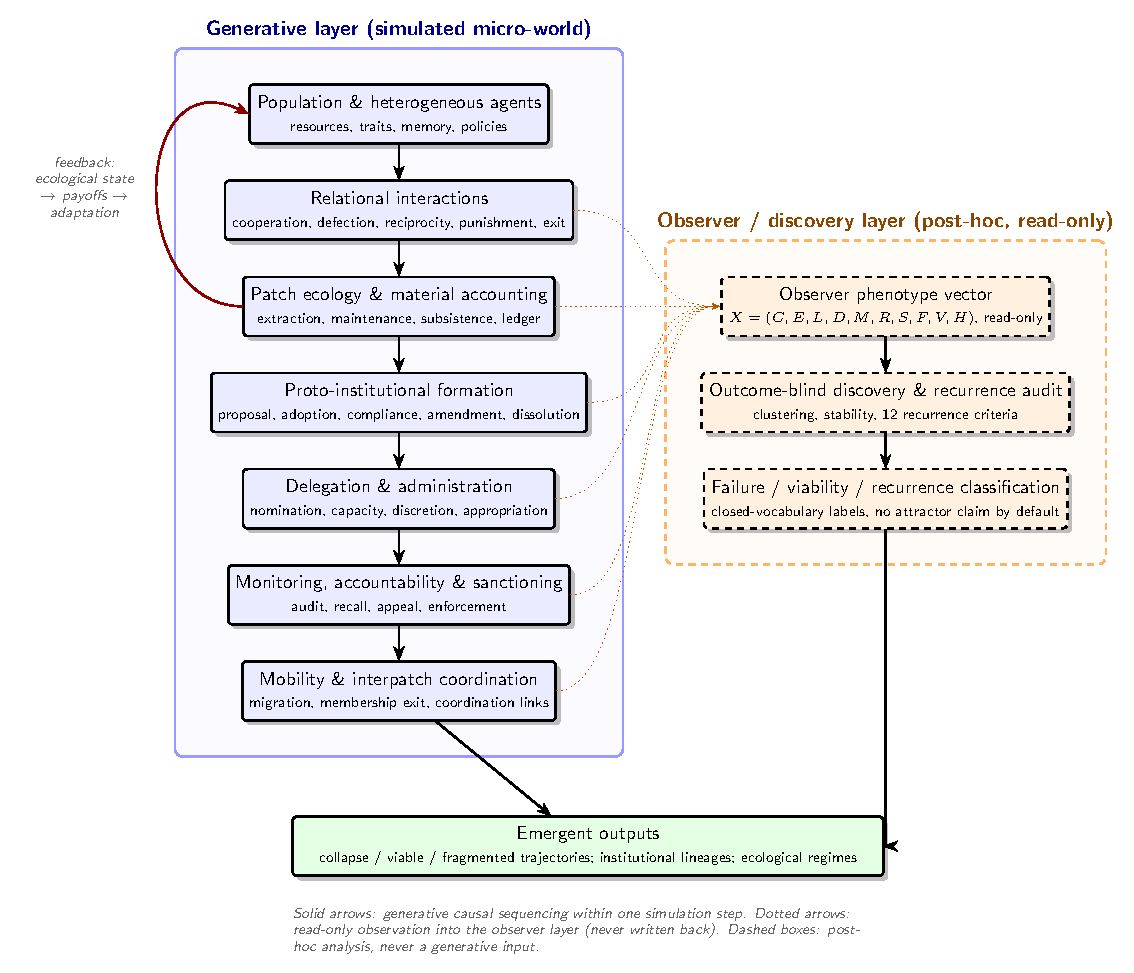
\includegraphics[width=\textwidth]{figures/main/conceptual_framework.pdf}
\caption{Conceptual framework: the generative layer (population,
relational interactions, patch ecology, proto-institutional formation,
delegation and administration, monitoring/accountability/sanctioning, and
mobility/interpatch coordination) versus the observer/discovery layer
(phenotype vector, outcome-blind discovery and recurrence audit, and
classification), kept structurally and visually separate throughout. Solid
arrows are generative causal sequencing within one simulation step; dotted
arrows are read-only observation into the observer layer, never written
back; the red feedback path is the sole channel by which ecological state
alters subsequent agent behavior. Originally authored for this paper
(\texttt{scripts/conceptual\_framework.tex}), structurally informed by
JUNE-style layered agent-based-model overview diagrams but drawn
specifically from this project's own architecture.}
\label{fig:conceptual-framework}
\end{figure}

\subsection{Agents, patches, resources, and networks}
\label{sec:agents-patches}

The population is heterogeneous by construction: every numeric trait is
drawn independently from its own configured distribution, never shared
across agents. Agents interact bilaterally over a dynamic relationship
network under a repeated cooperation/defection payoff grammar, observe
each other with bounded accuracy, retain a decaying memory of past
partners, and may punish a perceived defector at a cost. A second,
structurally independent action dimension governs each agent's ecological
behavior --- extraction, maintenance investment, or restraint --- directed
at one of a fixed number of local resource patches to which agents are
assigned once, at initialization, by a neutral rule. Each patch has its
own carrying capacity and logistic regeneration; extraction and
maintenance are resource-unit transactions rationed under a documented
allocation rule when simultaneous demand exceeds a patch's capacity to
serve it. Level 1.2 adds a structural mobility primitive
(\texttt{PatchSystem.migrate}) and, gated by their own flags, migration
and voluntary membership exit.

\subsection{Behavioral and institutional adaptation}
\label{sec:behavioral-adaptation}

Agents adapt via imitation (copying a peer's policy with probability
increasing in the peer's relative resource advantage) and low-rate
mutation --- never planning or lookahead. The two behavioral dimensions
(social and ecological) are, in the model's default configuration, given
independent imitation draws; a coupled mode exists but is not the
configuration used in the runs reported here. Institutions adapt on a
slower, structurally distinct channel: a locally shared rule
(\texttt{SharedRule}) is proposed, accumulates support, and is adopted or
rejected by a local threshold process; once active it is monitored,
enforced, and may be amended or dissolved; a dissolved rule's parameters
are retained (not discarded) as the sole source from which a later
reconstruction attempt may mutate. From Level 1.1, a rule may delegate
monitoring, record-keeping, sanction execution, maintenance coordination,
or interpatch communication to a nominated and selected delegate, whose
administrative capacity is built up only from realized task performance
(never assigned as a static trait) and who may exercise discretion ---
appropriation and effort withholding --- subject to accountability
(audit, recall, appeal). From Level 1.2, institutions may also be locally
observed by other patches (with noise, distortion, and delay), transmitted
component-wise across the existing coordination-link graph (with
mutation, recombination, or failure), competed for via migration, and
scaled across jurisdictions that grow, shrink, merge, fragment, or
dissolve.

\subsection{Institutional representation and lineage}
\label{sec:institutional-representation}

Each institution is represented by a fourteen-slot component bundle
(\texttt{InstitutionComponents}: proposal, adoption, contribution,
monitoring, sanction, appeal, recall, delegation, administration,
authority, amendment, memory, succession, coordination), of which twelve
are transmissible across the coordination-link graph and two remain
descriptive-only in this milestone. A full lineage record
(\texttt{InstitutionRecord}) tracks parentage, origin mechanism (fresh
proposal, component transmission, reconstruction, or recombination),
active jurisdiction, amendment history, transmission history, and
extinction time and reason. Lineage identifiers are allocated from a
per-simulation-run counter and are therefore unique only \textit{within}
one seed-run; \cref{sec:level12b} reports a genuine bug this created when
pooling lineage identity across the many independent seed-runs Level 1.2b
introduced, and its fix.

\subsection{Random-number substreams and reproducibility}
\label{sec:rng-substreams}

Every stochastic draw in the codebase passes through one explicit, seeded
random-number generator per run; no module calls an unseeded global
source. From Level 1.1b, an opt-in per-mechanism substream architecture
(\texttt{rng\_mode="mechanism\_substreams"}) is available and is
\textit{mandatory} for every causal (matched-seed) experiment in both
Level 1.2 and Level 1.2b, so that a paired comparison's random draws for
one mechanism are never coupled to another mechanism's own draws under
the same nominal seed. The default \texttt{"legacy\_single\_stream"} mode
remains the exact, byte-for-byte baseline for every non-causal run.

\subsection{Observer metrics and outcome classifications}
\label{sec:observer-metrics}

The observer layer is read-only with respect to the generative layer,
checked by an abstract-syntax-tree-based import-direction test: observer
modules may read logged state and events; they may never write back into
agent state, policies, payoffs, or the random-number stream. Two closed,
non-normative classification vocabularies are used throughout. An
all-outcome classification (\texttt{classify\_all\_outcome}) assigns each
seed-run exactly one of seven labels ---
\texttt{no\_institution}, \texttt{collapse}, \texttt{viable},
\texttt{persistent\_extractive}, \texttt{fragmented}, \texttt{transient},
\texttt{unclassified} --- by first-match-wins rule; every label is always
reported, including zero counts, so that a dominant outcome can never be
silently omitted from a summary. A five-label failure-trajectory
classification (\texttt{classify\_failure\_trajectory}, Level 1.2b only)
distinguishes \texttt{no\_collapse\_observed}, \texttt{transient\_%
dip\_recovered}, \texttt{collapse\_onset\_after\_last\_snapshot},
\texttt{late\_onset\_collapse}, and \texttt{sustained\_collapse} from a
coarse population/ecological-fraction series sampled every ten steps.
Neither vocabulary contains, or is derived from, any dissertation-side
concept.

The observer-only institutional phenotype vector
$X=(C,E,L,D,M,R,S,F,V,H)$ --- realized administrative capacity, effective
constraint, legitimacy (voluntary support), concentration of delegated
authority, institutional memory continuity, administrative appropriation
burden, institutional scale/reach, amendment flexibility, ecological/
demographic viability (two subparts, reported separately), and
within-community heterogeneity --- is computed once per seed-run, never
agent-visible and never a generative input anywhere. A dedicated
Level 1.2b audit (\cref{sec:level12b}) formally checked every dimension's
numerator, denominator, window semantics, missingness condition,
aggregation path, and construct type against six required criteria; no
dimension was removed, and the one genuine transparency gap it found
(inconsistent disclosure of whether a requested time window actually
changed a dimension's value) was fixed additively, without changing any
existing numerator, denominator, or computed value.

\subsection{Outcome-blind discovery procedure}
\label{sec:discovery-procedure}

The unit of analysis is one phenotype vector per seed-run, never per
institution and never per simulation step. Preprocessing compares three
missingness strategies (\texttt{complete\_case}, \texttt{mean\_impute},
\texttt{missingness\_indicator}) rather than silently choosing one, with
standardization always fit on the training split only. Three
structurally different clustering families are fit at every $k$ from 1
through 8 (a disclosed reduction from a fuller candidate menu; $k=1$ is
always fit and never treated specially, and no $k$, including $k=3$, is
privileged): a parametric Gaussian mixture model
\parencite{fraley2002model}, agglomerative hierarchical clustering, and
density-based \texttt{HDBSCAN} \parencite{campello2013density}, which
alone among the three permits unclustered noise points rather than
forcing every observation into some cluster. Model selection reports
silhouette \parencite{rousseeuw1987silhouettes}, Calinski--Harabasz,
Davies--Bouldin, cluster-size balance, and, for the Gaussian mixture,
Bayesian and Akaike information criteria and held-out log-likelihood side
by side, with no single metric deciding. Consensus is assessed via a
pooled co-assignment matrix, the variation of information, bootstrap
stability (resample-with-replacement adjusted Rand index against the
original fit; \cite{hubert1985comparing,benhur2002stability,efron1993bootstrap}),
and pairwise algorithm agreement.

Twelve preregistered recurrence criteria (\texttt{minimum\_cluster\_size},
\texttt{cross\_seed\_recurrence}, \texttt{cross\_algorithm\_support},
\texttt{bootstrap\_stability}, \texttt{co\_assignment\_internal\_%
consistency}, \texttt{distinctness\_from\_noise}, \texttt{missingness\_%
strategy\_robustness}, \texttt{parameter\_condition\_diversity},
\texttt{temporal\_persistence\_of\_members}, \texttt{non\_degenerate\_%
cluster\_fraction}, \texttt{k\_selection\_non\_privileged\_support},
\texttt{independent\_of\_single\_lineage}) are evaluated unconditionally
for every candidate cluster, with no short-circuiting, and combined by
strict conjunction --- a candidate is recurrent only if it passes all
twelve, never a majority. None of the twelve references cluster count or
identity. Level 1.2b's own audit (Work Package H, \cref{sec:level12b})
re-examined every criterion's construct, unit of analysis, and redundancy
under the larger joint design, found and fixed a genuine cross-seed-run
lineage-identifier collision (\cref{sec:institutional-representation}),
and froze a versioned, hashed specification before any discovery result
was seen.

Level 1.2b additionally defines a closed six-label discovery-verdict
vocabulary (\texttt{insufficient\_evidence}, \texttt{failure\_dominated},
\texttt{unstable}, \texttt{one\_config}, \texttt{continuum},
\texttt{multi\_config}), evaluated first-match-wins: whether sample size
and a defined headline $k$ exist at all; whether clustering merely
re-derives the model's own failure/success split; whether either
bootstrap or algorithm-agreement stability clears a 0.3 floor (either is
sufficient, since they measure different kinds of robustness); whether
any $k\geq2$ clears a 0.15 silhouette floor; and, if so, whether three or
more evaluated $k$'s sit within 0.05 silhouette of the best $k$
(\texttt{continuum}) versus a single, clearly dominant peak
(\texttt{multi\_config}). This vocabulary is the direct methodological
response to a documented limitation of silhouette-based model selection
alone: a genuine discrete two-cluster structure and a smooth, gap-free
continuum with one dominant bisection can produce statistically
indistinguishable single-peaked silhouette curves. Neither Level 1.2's
nor Level 1.2b's discovery pipeline can, by itself, prove that a sharp
verdict reflects true discreteness; a \texttt{continuum} verdict is
correspondingly read as evidence of gradedness, not merely as an absence
of a sharp answer.

\subsection{Historical pressure, entrenchment, and legitimacy mechanisms}
\label{sec:historical-mechanisms}
\label{sec:observer-metrics-l13}

Level 1.3 adds history as a generative mechanism, not merely a
richer observer-side measurement. Three pressure channels ---
\textit{security pressure} ($W_t$), \textit{bargaining pressure} ($B_t$),
and \textit{coordination-complexity pressure} ($X_t$) --- are each wired
through two of six candidate transmission primitives shared across
channels: \texttt{pressure\_adjusted\_probability} (a pressure-scaled
adjustment to an existing stochastic decision, e.g.\ monitoring or
sanctioning likelihood) and \texttt{pressure\_adjusted\_scale} (a
pressure-scaled adjustment to an existing continuous quantity, e.g.\
contribution size or delegation scope). Every channel defaults to a
verified no-op; enabling a channel changes only the specific decision or
quantity its own transmission primitives touch, confirmed by regression
test against Level 1.2b's own unmodified behavior at every default setting.
\textit{Institutional entrenchment} is a single additional state variable,
an age-dependent multiplier on the cost or difficulty of amending or
dissolving an active rule, driven by \texttt{entrenchment\_maturation\_%
steps}, itself off/moderate/strong. \textit{Dual legitimacy} extends the
existing legitimacy dimension into two independently accumulated, costly,
and fallible ledgers --- \textit{performance legitimacy} ($L_P$, earned
from realized institutional outcomes) and \textit{procedural legitimacy}
($L_R$, earned from realized procedural/reciprocal fairness) --- each
independently enableable.

The observer layer adds two post hoc composites, $S_{\text{obs}}$ and
$Z_{\text{obs}}$, computed exclusively from existing Level 1.2/1.2b/1.3
observer fields and never read back into the generative layer. $S_{\text{%
obs}}$ is the unweighted mean of five components: \texttt{delegation},
\texttt{administrative\_function}, \texttt{monitoring}, \texttt{interpatch\_%
coordination}, and \texttt{performance\_legitimacy}. $Z_{\text{obs}}$ is
the unweighted mean of three components: \texttt{accountability},
\texttt{bargaining\_participation}, and \texttt{procedural\_legitimacy}.
The two composites share zero component dimensions by construction,
confirmed by direct inspection of \texttt{observer/sz\_obs.py}'s own
constants (\cref{sec:level13b-measurement}). We are explicit that
$S_{\text{obs}}$ and $Z_{\text{obs}}$ are this project's own observer-side
constructs, built without reference to and structurally firewalled from
the dissertation's SEM latent factors $S$ and $Z$; any correspondence
between them is a substantive question this paper's own discussion takes
up (\cref{sec:disc-triangulation}), never an assumption built into either
construction.

\subsection{Sequencing, persistence, and sham-controlled causal intervention}
\label{sec:sequencing-and-intervention}

Level 1.3 tests pressure-channel \textit{ordering} via a matched factorial
crossing onset order (\texttt{security\_first}, \texttt{bargaining\_first},
\texttt{coevolution}) with entrenchment and legitimacy conditions, holding
each channel's total cumulative exposure matched across orderings so that
any observed difference reflects onset timing and sequence, not total
pressure magnitude. Level 1.3b adds a third counterfactual pressure-history
transform, \texttt{equalize\_pressure\_series} (flattening a channel's
realized series to its own mean, preserving cumulative exposure exactly
while destroying temporal shape), alongside the two Level 1.3 already
had (\texttt{remove\_pressure\_history}, \texttt{reverse\_pressure\_%
history}).

Windowed persistence diagnostics (\texttt{observer/historical\_%
persistence.py}, new at Level 1.3b) partition a run's own duration into
early/middle/late/final-sustained windows and compute, per window,
within-window means and variances, early-to-middle and middle-to-late
displacement, a convergence/divergence slope, and a closed five-label
persistence classification (\texttt{transient\_differentiation},
\texttt{historical\_hysteresis}, \texttt{pressure\_dependent\_response},
\texttt{entrenched\_path\_dependence}, \texttt{no\_detectable\_%
differentiation}).

Level 1.3b's own Stage 6 adds a sham-controlled, matched-seed causal
intervention design, the strongest causal evidence this project has
produced for or against historical path dependence. For each of 12 matched
seeds, six arms are compared: a \texttt{no\_intervention\_control}; a
\texttt{sham\_identical\_state\_copy} (the checkpoint/fork machinery
itself, with no history actually altered --- this arm must match the
control byte-for-byte, or the fork machinery, not history, would be
responsible for any divergence seen elsewhere); and four real
interventions (\texttt{pressure\_memory\_only}, \texttt{entrenchment\_%
only}, \texttt{legitimacy\_history\_only}, \texttt{all\_history}), each
resetting or erasing a specific piece of accumulated historical state at a
mid-run checkpoint while leaving the rest of the run's own machinery
untouched. \texttt{core/state\_checkpoint.py} supplies the underlying
\texttt{run\_partial}/\texttt{fork}/\texttt{finish} primitives; a genuine
\texttt{copy.deepcopy}/frozenset-iteration-order bug in an early build of
this machinery was caught by the sham arm's own byte-identical requirement
before any real Stage 6 run completed (\cref{sec:level13b-limitations}),
and fixed by rebuilding each intervention arm fresh from an independent
\texttt{Simulation(config)} construction (already proven byte-identical to
a live fork) rather than forking a live object.

\subsection{Extended decision-gate vocabulary}
\label{sec:decision-gate-extended}

Level 1.3b extends Level 1.2b's own closed six-label discovery-verdict
vocabulary (\cref{sec:discovery-procedure}) to eight labels for the
historical-extension milestones specifically, distinguishing among
possible historical-effect outcomes rather than only discreteness outcomes:
\texttt{no\_effect}, \texttt{pressure\_responsive\_nonhistorical} (responds
to pressure magnitude but not temporal order/history), \texttt{transient}
(differentiation appears but reconverges), \texttt{persistent\_continuum}
(persistent path dependence on a continuous gradient), \texttt{two\_%
families}, \texttt{three\_families}, \texttt{four\_or\_more\_families}, and
\texttt{inconclusive}. This vocabulary was frozen, with an explicit note
that its own discovery pipeline must not be biased toward
\texttt{three\_families} as a default, before any Stage 3+ Level 1.3b run
executed. Ruling out the discrete-family labels (\texttt{two\_%
families}/\texttt{three\_families}/\texttt{four\_or\_more\_families}) reuses
Level 1.2b's own frozen \texttt{classify\_discovery\_verdict} function
unmodified, applied to Level 1.3b's own Stage 7 discrete-candidate fit ---
the same discipline Level 1.3 itself already followed, now extended one
milestone further, so that no discreteness rule was ever authored, or
re-authored, after either milestone's own data was already in hand.

\subsection{Preregistration and confirmation logic}
\label{sec:preregistration-logic}

All four milestones freeze a hashed manifest before Stage/Work-Package
execution begins --- mechanism-activation flags, sample sizes,
discovery-pipeline commitments, recurrence criteria, and
random-number-generator discipline for Level 1.2; feasibility-ratio
definitions, ecological strata, institutional bounds, burn-in windows,
run-count arithmetic, and a confirmation rule for Level 1.2b; pressure-
channel/entrenchment/legitimacy activation ranges, sample sizes, and
stage-by-stage design for Level 1.3; and, for Level 1.3b, the eight
hypotheses of \cref{sec:level13b}, the eight-label decision-gate vocabulary
of \cref{sec:decision-gate-extended}, and an explicit
\texttt{DECISION\_GATE\_DO\_NOT\_PREFER = "F\_three\_families"} note scoped
to mean only that the discovery pipeline's own default must not be biased
toward three families, not that three families is disqualified as a
genuine finding if the evidence actually supports it. Every subsequent
stage script recomputes the manifest's cryptographic hash and refuses to
proceed on any mismatch, making the "never alter the model or rerun a
search merely because the outcome differs from an expected answer"
discipline mechanically checkable rather than a stated intention. Level
1.2b's confirmation rule --- if discovery supports no discrete candidates,
including a \texttt{continuum} verdict, the fresh confirmation sample
replicates the null finding rather than being used to manufacture a
candidate to test --- is inherited unmodified by Level 1.3b's own Stage 8
confirmation design. \Cref{sec:level12b,sec:level13,sec:level13b} report
how this rule was actually applied at each milestone.

Both Level 1.3 and Level 1.3b's own governing specifications were
authored, at length, in an earlier working session whose exact verbatim
text is not recoverable after a later context compaction; every downstream
document (preregistration modules, scientific notes, decision-gate reports)
discloses this explicitly in its own text rather than presenting a
reconstructed hypothesis list or evidence-table schema as a verbatim
transcription. This paper reports the reconstructed hypotheses and
findings the source project itself worked from, with the same disclosure
carried forward rather than smoothed over (\cref{sec:limitations}).
